\section*{Filter Example}
\addcontentsline{toc}{section}{Filter Example}

The following example is taken from section 9.5.2 of reference \cite{opt}. The
load impedance is a series inductor of value \SI{2.3}{\henry}, a shunt capacitor
of value \SI{1.2}{\farad} and a parallel resistor (the load resistance) of value
\SI{1}{\ohm}. Thus, we can express $z(s) = 2.3s + 1/(\frac{1}{1.2s} +
\frac{1}{1})$ (note the lower case usage of z for the load). I have used the
code included in appendix \ref{sec:appendix_a_matlabtextregistered} to generate
the following filter design:

\begin{figure}[H]
    \centering
    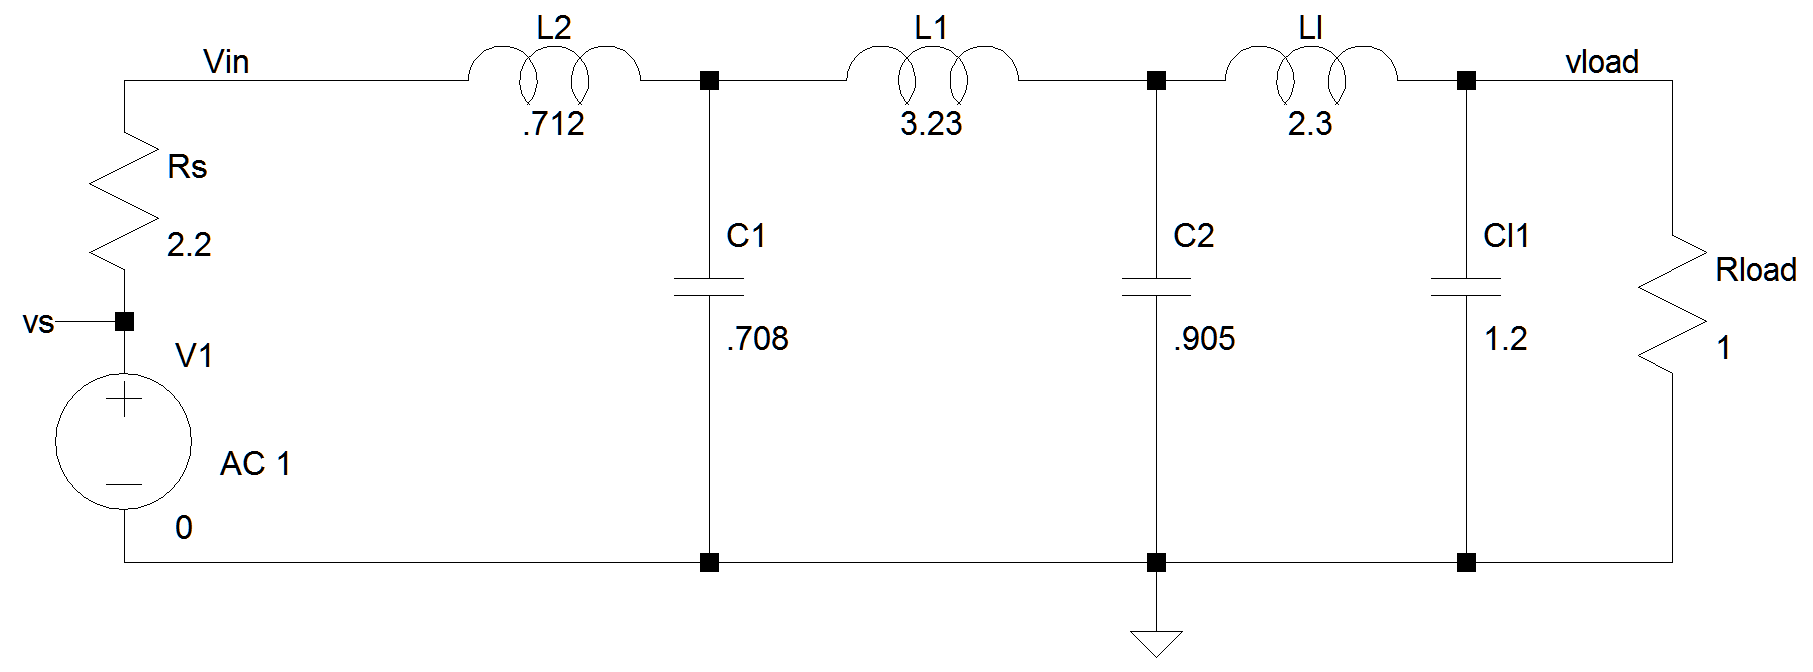
\includegraphics[width=0.8\linewidth]{../img/Load.PNG}
    \caption{Schematic determined by the SRFT}
    \label{fig:load}
\end{figure}

The results of having had simulated this network in
LTSpice\textsuperscript{\textregistered} are given below:

\begin{figure}[H]
    \centering
    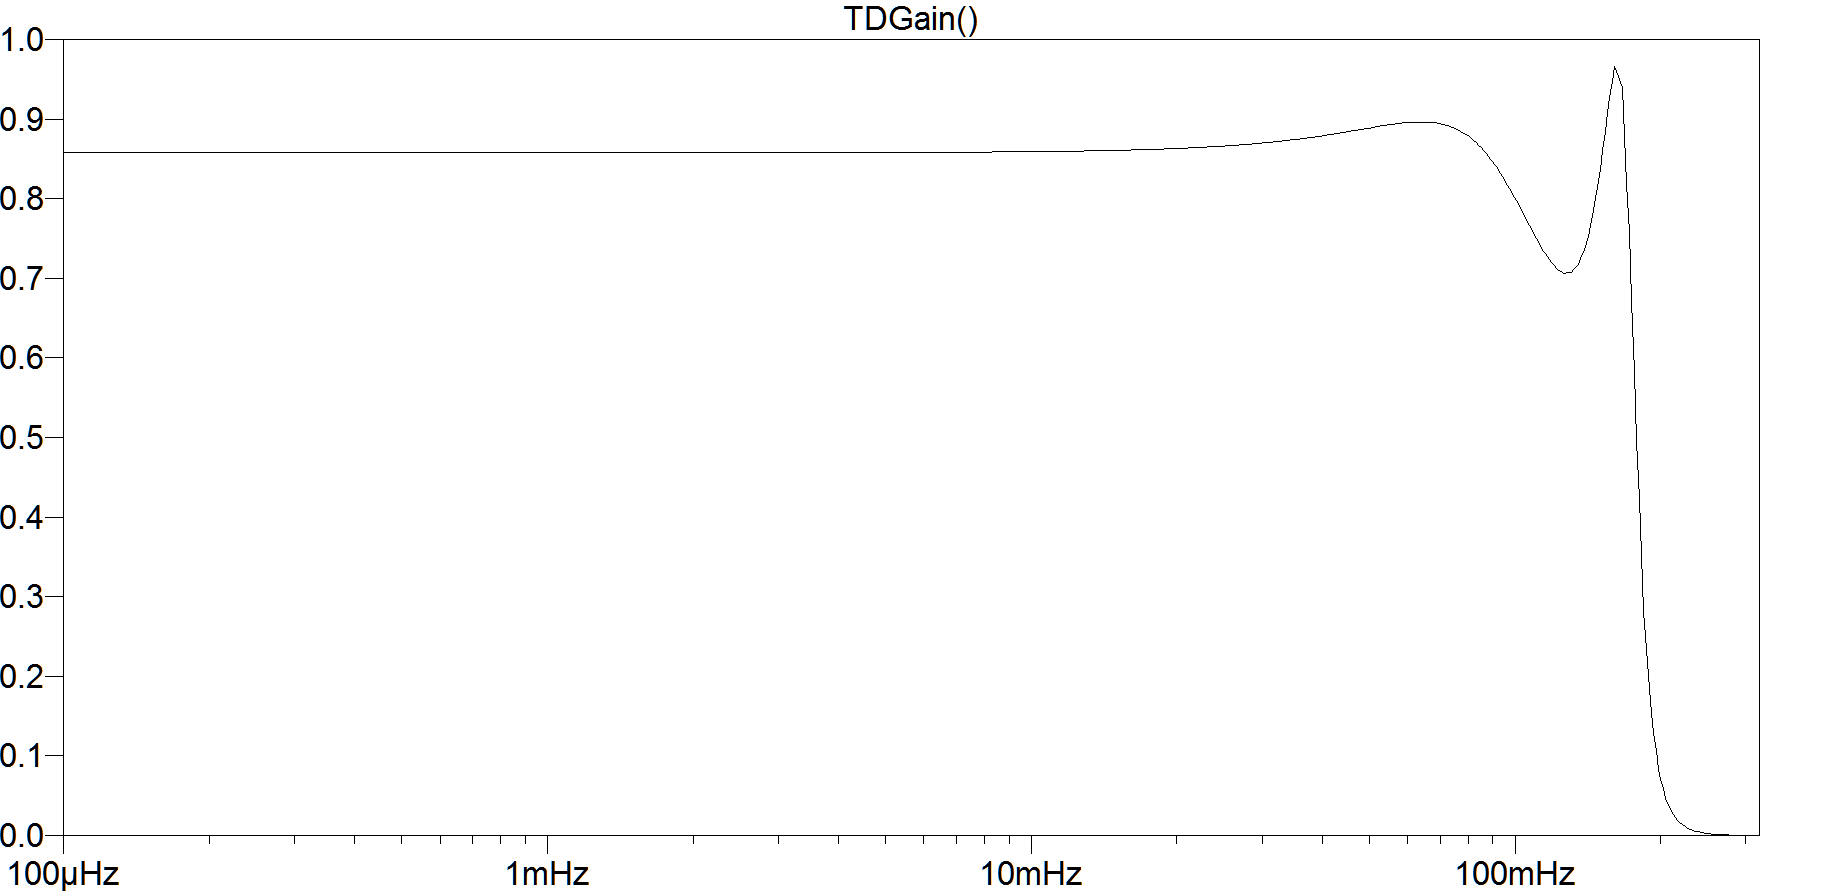
\includegraphics[width=0.8\linewidth]{../img/LTSpiceResults.png}
    \caption{Results of having had simulated the network of figure
    \ref{fig:load} in LTSpice\textsuperscript{\textregistered}}
    \label{fig:LTSpiceResults}
\end{figure}

These component values are currently returned to the
MATLAB\textsuperscript{\textregistered} command line window once the entire SRFT
has been completed. The command line output for this example is shown in the
figure below.

\begin{figure}[H]
    \centering
    \includegraphics[width=0.8\linewidth]{../img/matlabclc.png}
    \caption{Output of the SRFT algorithm in the
    MATLAB\textsuperscript{\textregistered} command line window}
    \label{fig:matlabclc}
\end{figure}
This simulation can be compared to the goal and obtained transducer gain (shown
below):

\begin{figure}[H]
    \centering
    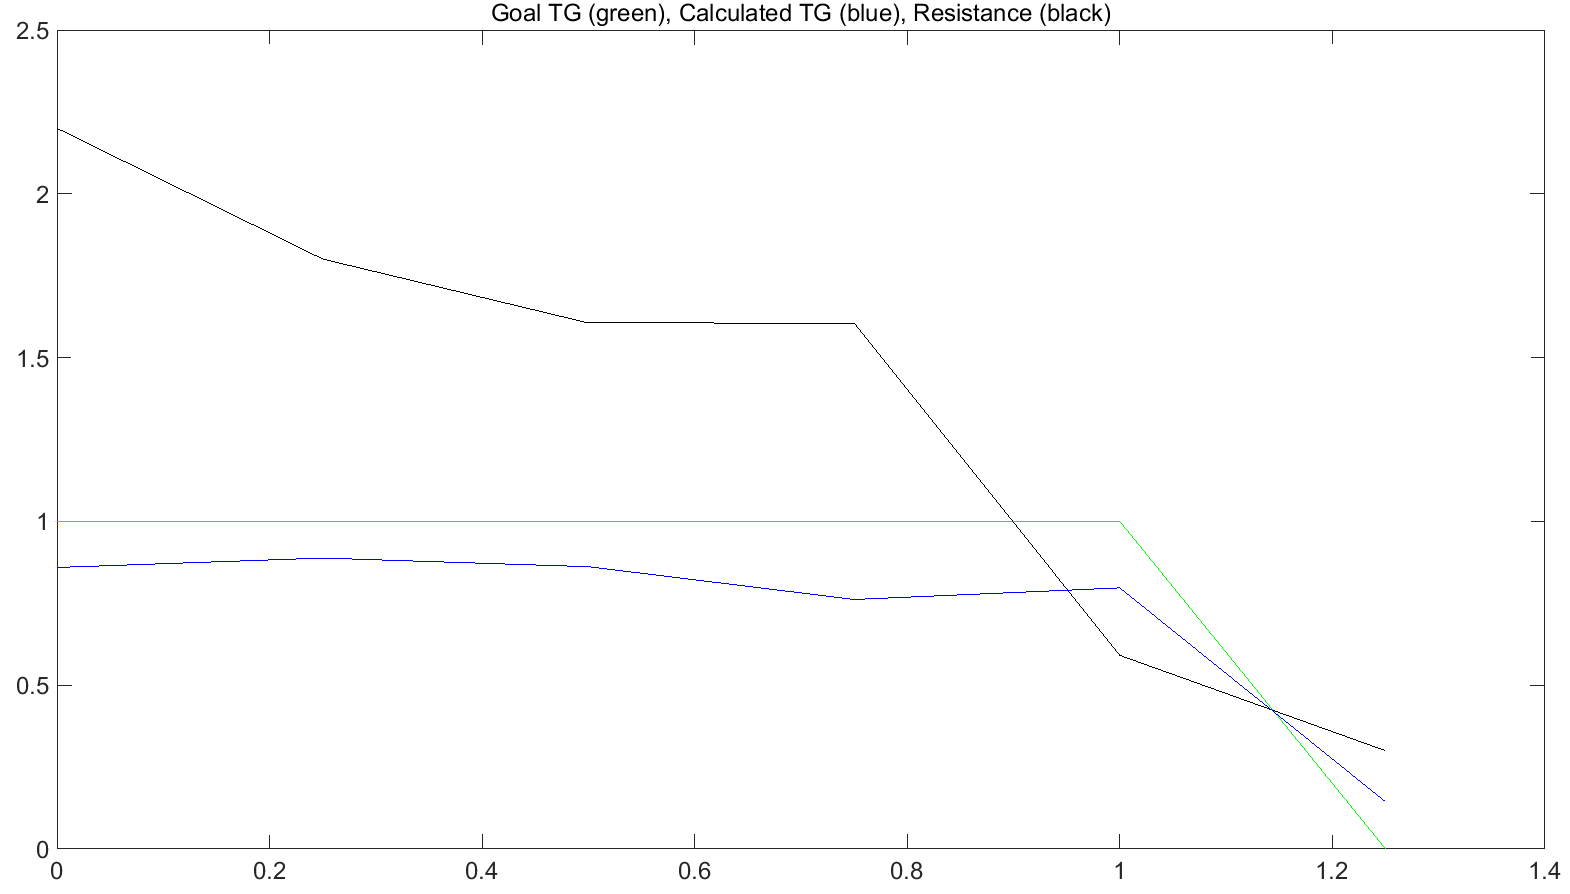
\includegraphics[width=.8\linewidth]{../img/OptimumGain.png}
    \caption{MATLAB\textsuperscript{\textregistered} calculated piecewise
    resistance (black), optimum/goal gain function (green) and numerically-obtained
gain function (blue). The 6 break points ($\omega = 0,.25,.5,.75,1.0,1.25$) are
clearly visible in the piecewise resistance plot. The same vertical axis was
used for both the transducer gain and the resistance plot. The resistance
vertical axis
has units of ohms and the transducer gain is normalized to one (power delivered
to the load is the same as the available power from the source); the horizontal
axis has units of \SI{}{\radian\per\second}}
    \label{fig:../img/OptimumGain}
\end{figure}

The MATLAB\textsuperscript{\textregistered} results were obtained assuming 6
break frequencies. $\omega = 0,.25,.5,.75,1.0,1.25$. There are discrepancies
that exist between the LTSpice\textsuperscript{\textregistered} results and the
MATLAB\textsuperscript{\textregistered} results. There is good reason for this.
One reason is that the MATLAB\textsuperscript{\textregistered} results were
obtained using component values that were precise to within the numerical precision of
the calculations. A more significant reason for the difference, however, is that
the MATLAB\textsuperscript{\textregistered} implementation of the SRFT only
calculates the transducer gain at select points between the break points. The
LTSpice\textsuperscript{\textregistered} results are solved over a more
continuous bandwidth. 

The reason for the seeming discrepancy between the horizontal axes is that the
LTSpice\textsuperscript{\textregistered} results are plotted against linear
frequency (\SI{}{\hertz}) while the MATLAB\textsuperscript{\textregistered}
results are plotted against angular frequency (\SI{}{\radian\per\second}).

So far, no microwave circuit has been designed. However, this topology lends
itself well to design using open stubs on microstrip. All that would be needed
would be to transform the lumped components into transmission line components
using Kuroda's identities (to turn all inductors into capacitors, realizing open
shunt stubs instead of series short stubs) and Richard's transformations to turn
shunt capacitors into open shunt stubs of $\lambda/8$ length (\SI{45}{\degree}).
Time, unfortunately, did not permit for this. The code generation took quite
some time and it is not yet optimal. Future improvements are discussed below.
